\section{K-means Clustering}
To identify distinct patterns in health trajectories based on frailty, I employ k-means clustering, a widely used unsupervised machine learning technique \citep{macqueen1967}. K-means clustering partitions $n$ observations into $k$ clusters, where each observation belongs to the cluster with the nearest mean (cluster centroid), serving as a prototype of the cluster \citep{hartigan1979}. As \citet{hastie2009} note, ``The K-means algorithm is simple and fast, which accounts for its popularity.'' The frailty is first turned into a vector for those aged 50 to 60 with a 2-year step size due to data availability. Essentially, I am clustering individuals into groups that are as similar as possible in terms of their health trajectories (not just levels at a fixed age).

It is crucial to identify the optimal number of clusters ($k$), and I use two methods common in the literature to inform this decision: the elbow method and the silhouette method.

\subsection{Elbow Method}
The elbow method plots the within-cluster sum of squares (WCSS) against the number of clusters. As $k$ increases, the WCSS typically decreases, with the rate of decrease often showing a clear ``elbow'' point. This point, where additional clusters yield diminishing returns in reducing WCSS, suggests an optimal $k$ value \citep{kodinariya2013}. The method provides a visual tool for determining the most efficient number of clusters, balancing model complexity with explanatory power.

\begin{equation}
\mathrm{WCSS} = \sum_{i=1}^{k} \sum_{x \in C_i} \lVert x - \mu_i \rVert^2
\end{equation}

The elbow method showed a noticeable elbow at $k=3$, suggesting diminishing returns for higher $k$ values.

\begin{figure}[ht]
    \centering
    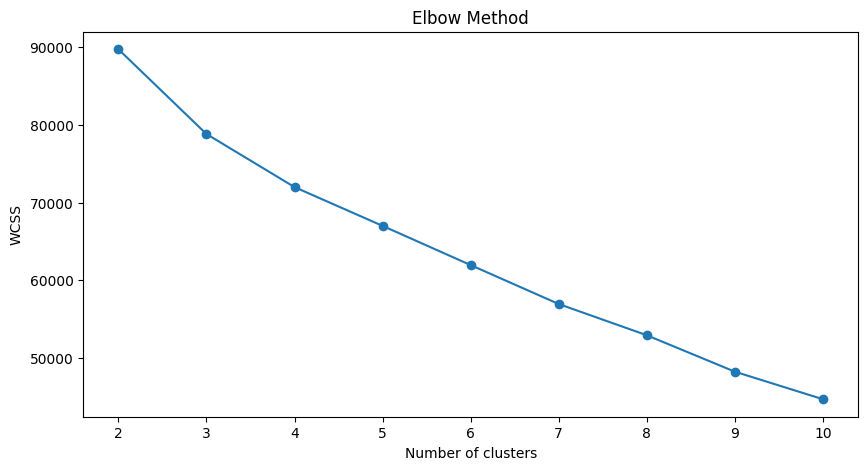
\includegraphics[width=0.8\textwidth]{figures/fig-007.png}
    \caption{Elbow method plot (extracted from the original dissertation PDF).}
    \label{fig:elbow}
\end{figure}

\subsection{Silhouette Method}
The silhouette method measures how similar an object is to its own cluster compared to other clusters \citep{rousseeuw1987}. Silhouette scores range from -1 to 1, with higher values indicating better-defined clusters. By plotting average silhouette scores against different $k$ values, I can identify the number of clusters that maximizes the score, suggesting optimal cluster separation and cohesion.

In my analysis, the silhouette method typically produced a concave shape, with relatively higher scores for lower $k$ values. Based on these results, I selected $k=3$ as an optimal midpoint between parsimony and fit.

\begin{figure}[ht]
    \centering
    
\includegraphics[width=0.8\textwidth]{figures/fig-008.jpg}
    \caption{Silhouette diagnostics (extracted from the original dissertation PDF).}
    \label{fig:silhouette}
\end{figure}
